\begin{figure*}[t]
\centering
\small
\noindent\textbf{Three research cases, five decision stages}\par\vspace{2pt}
\noindent\textcolor{TraceSlate}{\scriptsize Observation $\rightarrow$ Hypothesis $\rightarrow$ Investigation $\rightarrow$ Action $\rightarrow$ Validated outcome}\par\vspace{3pt}
\setlength{\tabcolsep}{3pt}
\renewcommand{\arraystretch}{1.18}
\begin{tabularx}{\textwidth}{@{}p{0.055\textwidth}X X X X X@{}}
\toprule
& \textbf{Observation} & \textbf{Hypothesis} & \textbf{Investigation} & \textbf{Action} & \textbf{Validated outcome}\\
\midrule
\textbf{T04}
&
\centering
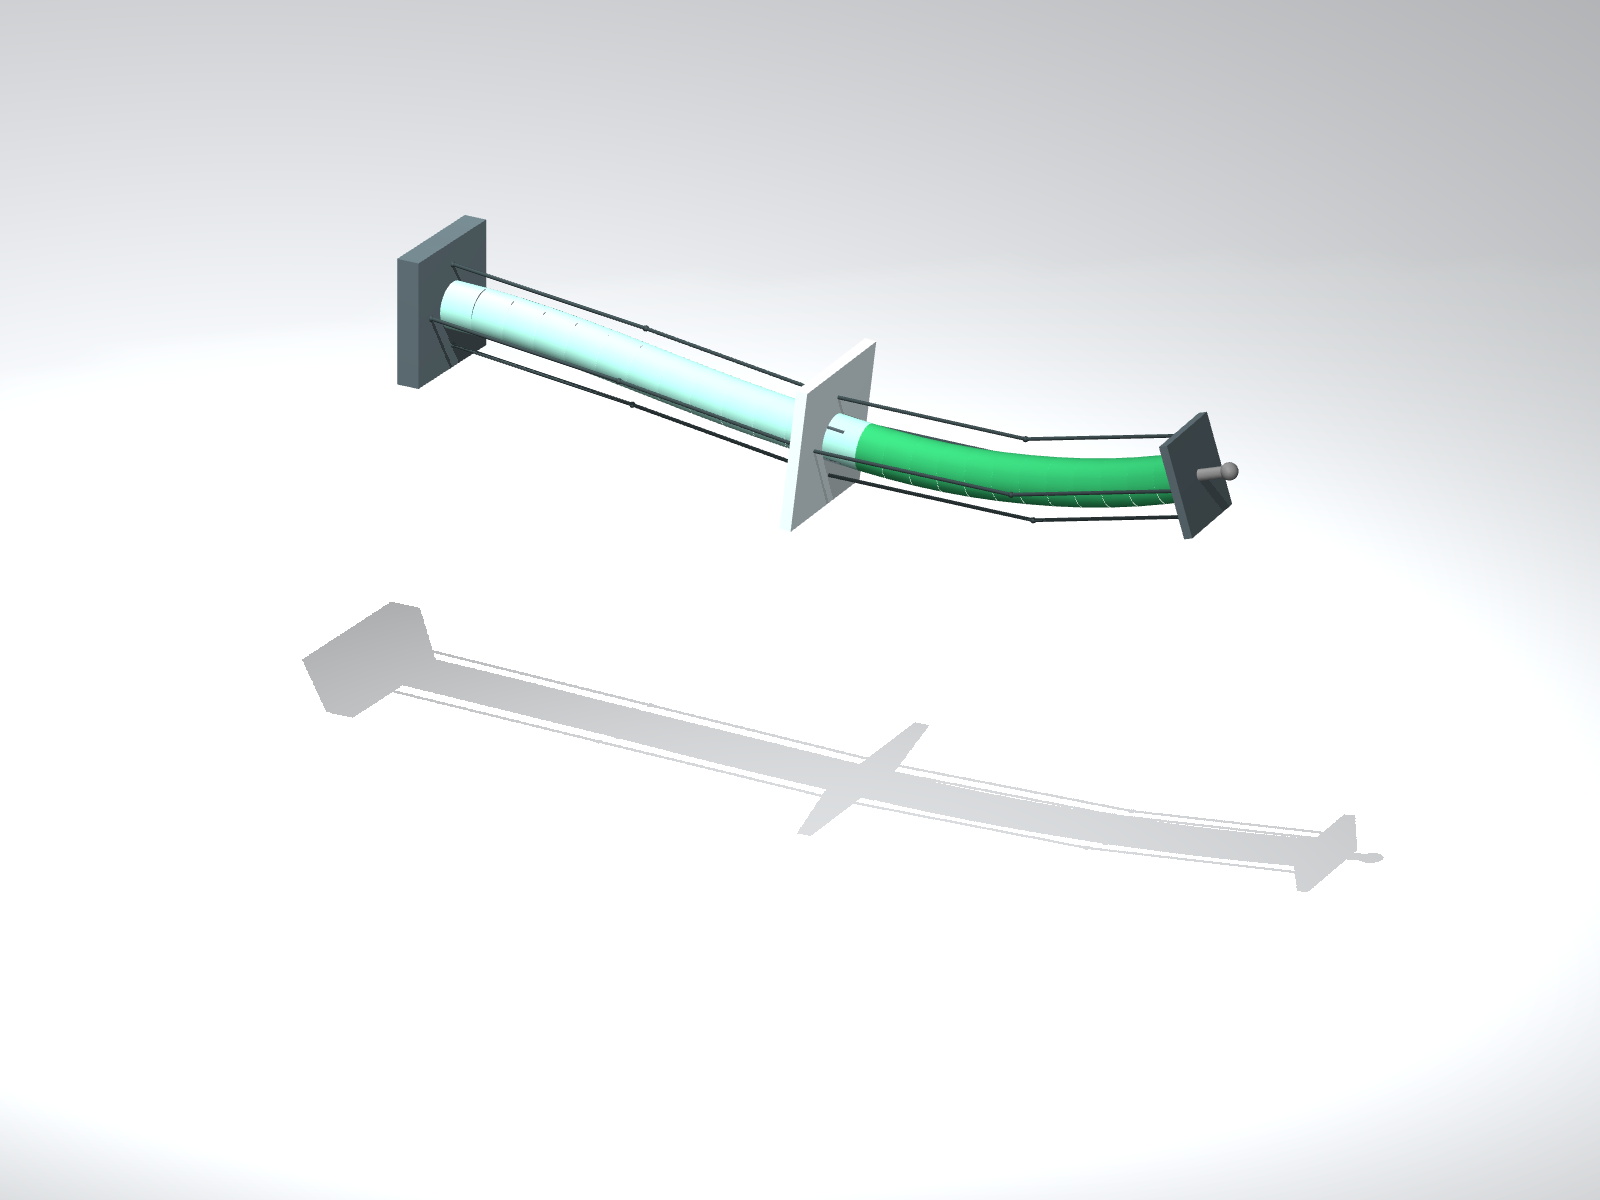
\includegraphics[width=\linewidth,height=0.60in,keepaspectratio]{figures/native/t04_earlier_route.png}\par
\scriptsize All-4~N initialization gives an inadmissible trial.
&
\scriptsize The immediate bottleneck is the reference initialization at the boundary, not the tracking objective.
&
\scriptsize Restart from the time-zero equilibrium; move boundary tensions from 0.20 to 0.21~N; construct an 89-point bank.
&
\centering
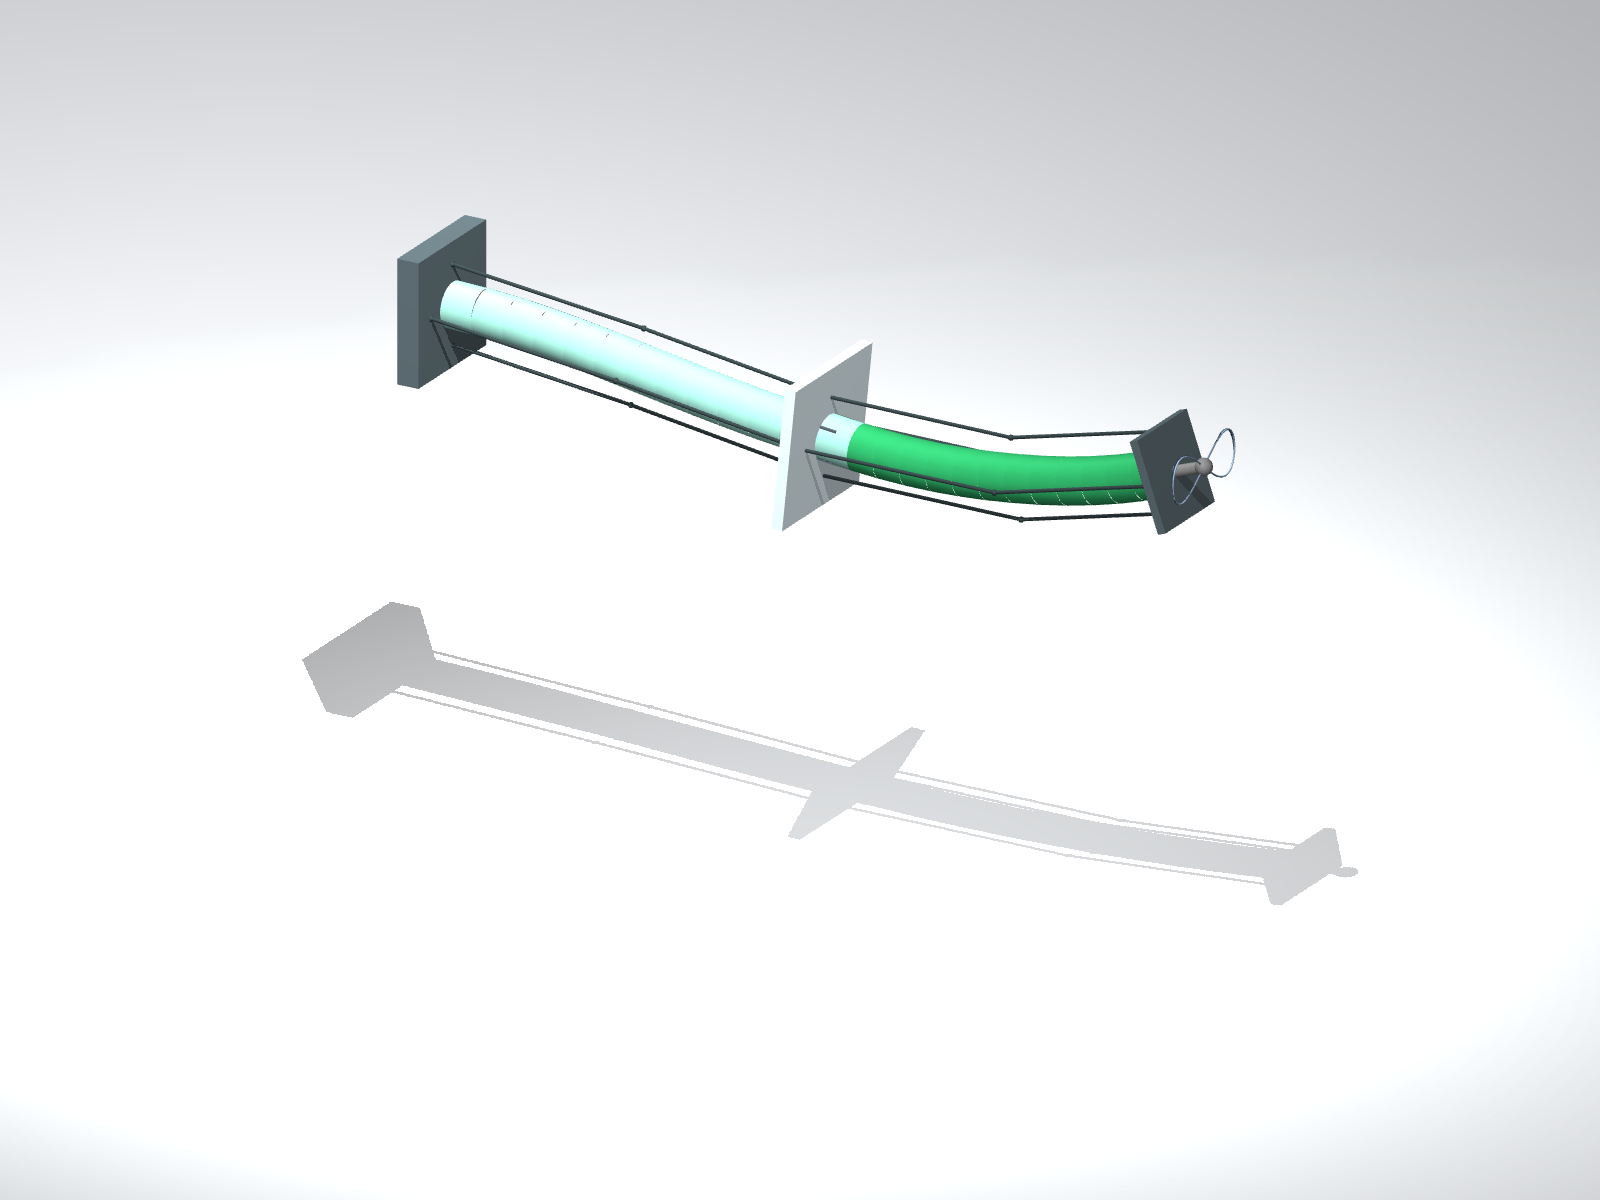
\includegraphics[width=\linewidth,height=0.60in,keepaspectratio]{figures/native/t04_final.png}\par
\scriptsize Use the equilibrium-consistent bank and interior seed.
&
\centering
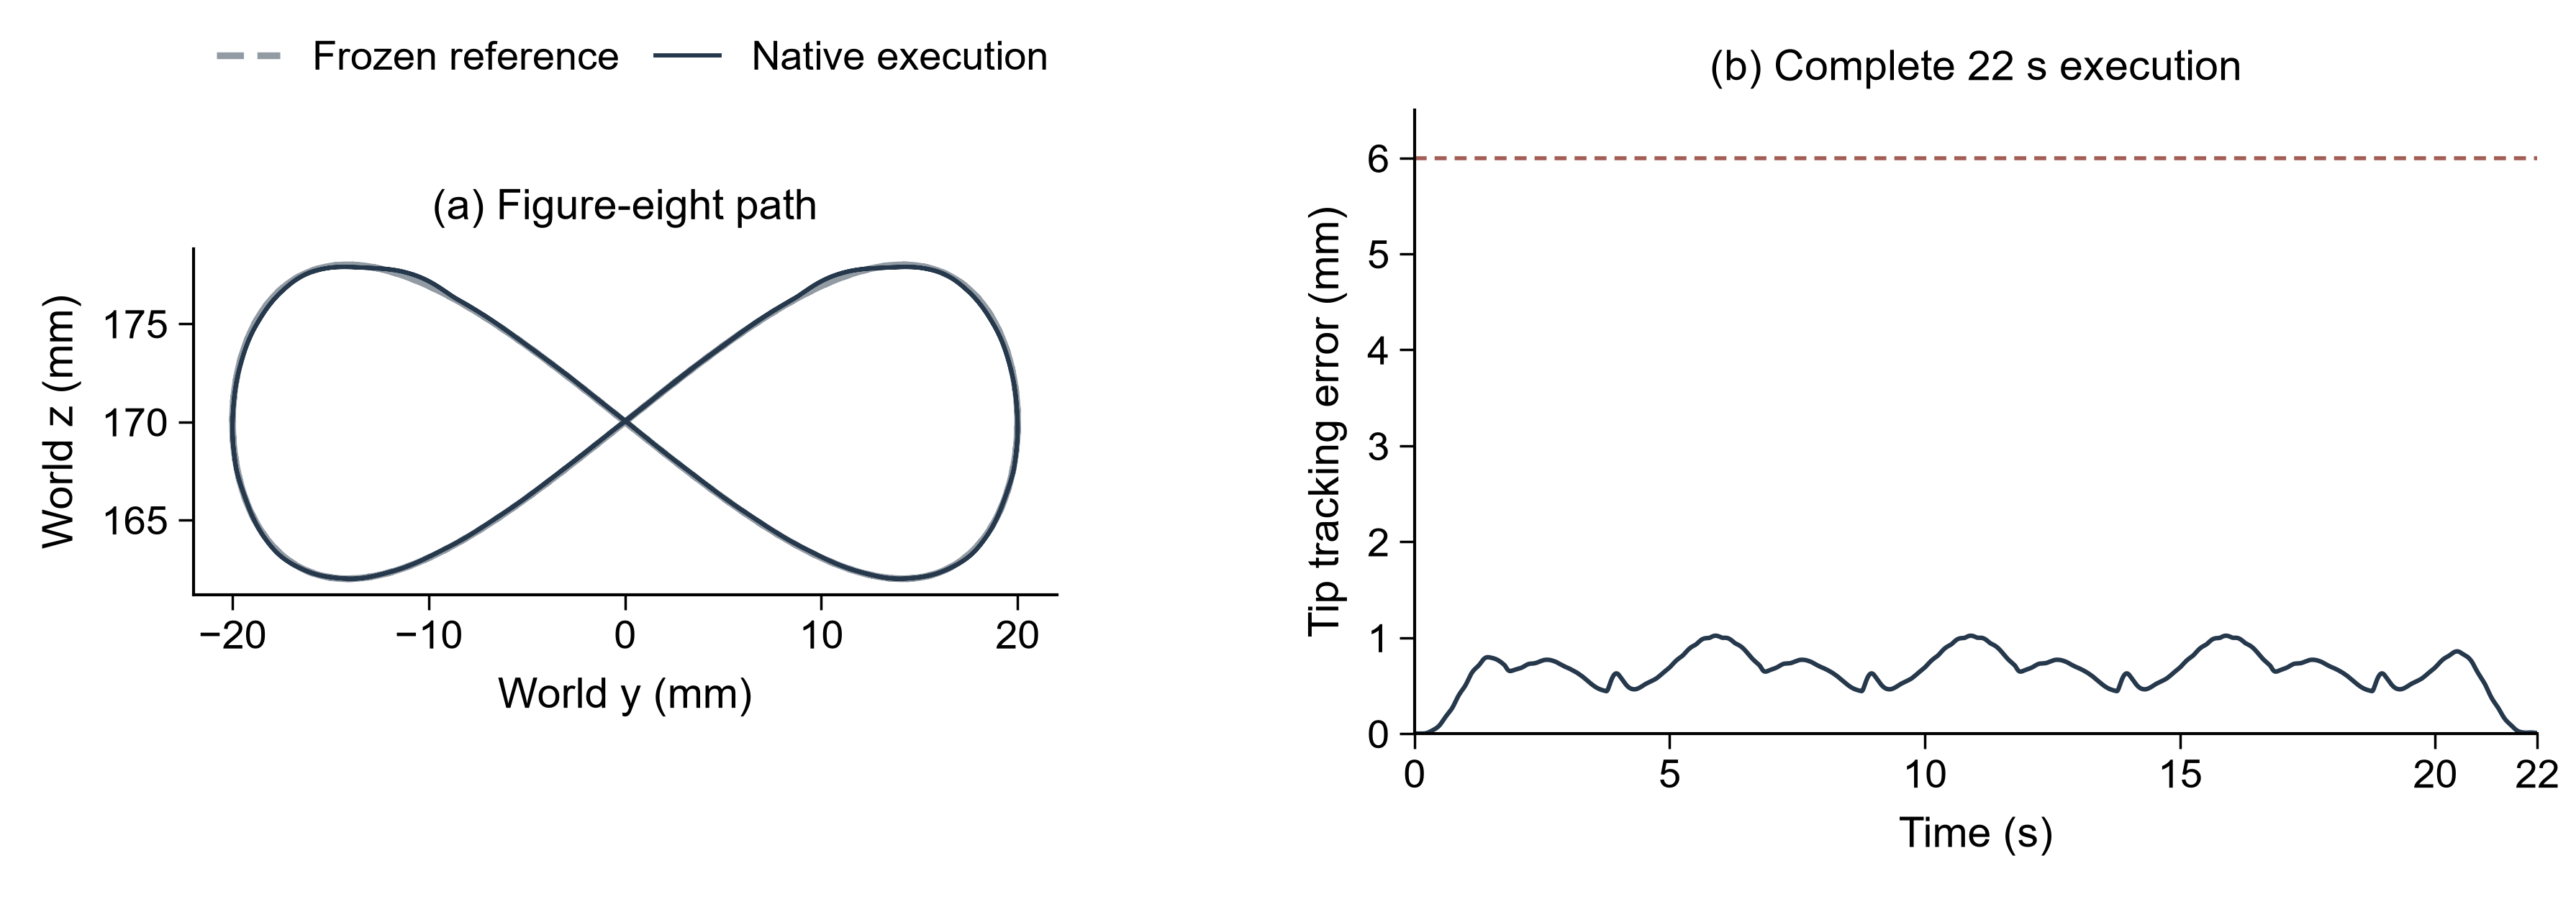
\includegraphics[width=\linewidth,height=0.60in,keepaspectratio]{figures/native/t04_tracking.png}\par
\scriptsize 22-s, two-cycle tracking; RMSE 0.688~mm; maximum error 1.021~mm.
\\
\midrule
\textbf{T07}
&
\centering
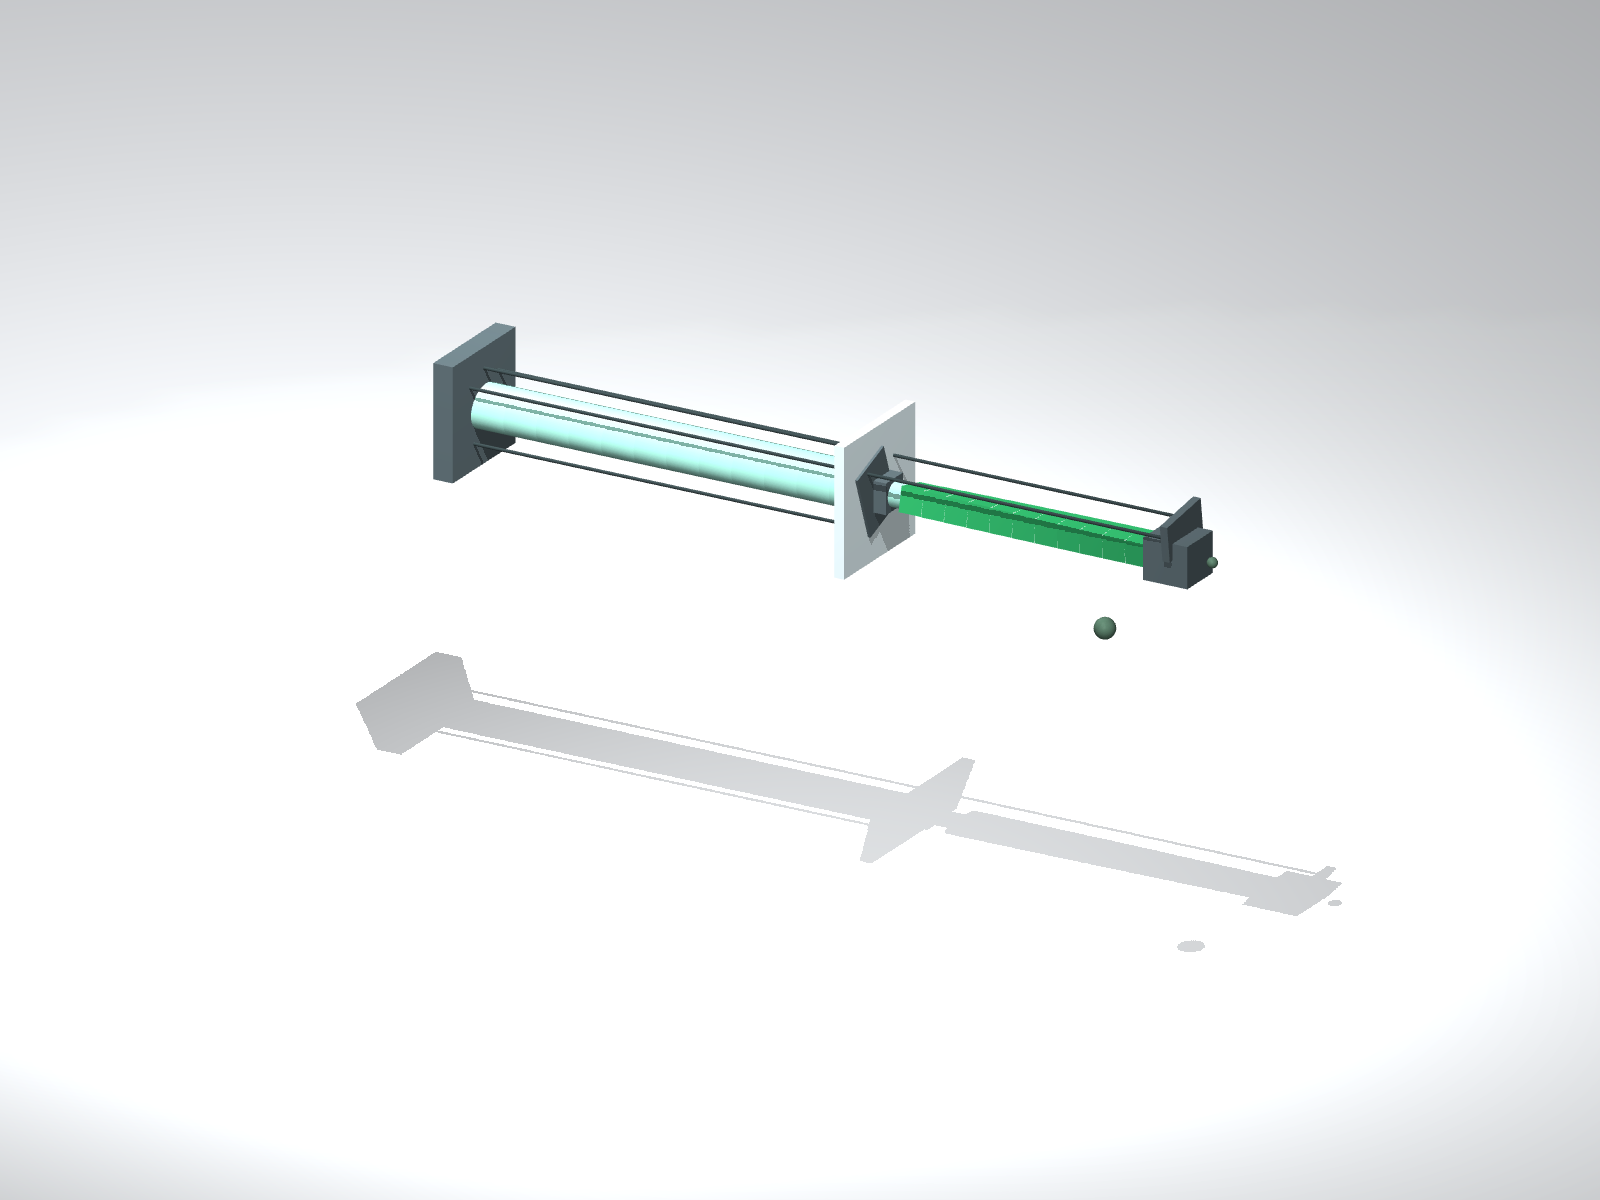
\includegraphics[width=\linewidth,height=0.60in,keepaspectratio]{figures/native/t07_ellipse_root.png}\par
\scriptsize Anisotropic root limits the shared task set.
&
\scriptsize The common morphology is constrained by root geometry as well as control.
&
\scriptsize Compare a rounded root and routing revision against all four required conditions.
&
\centering
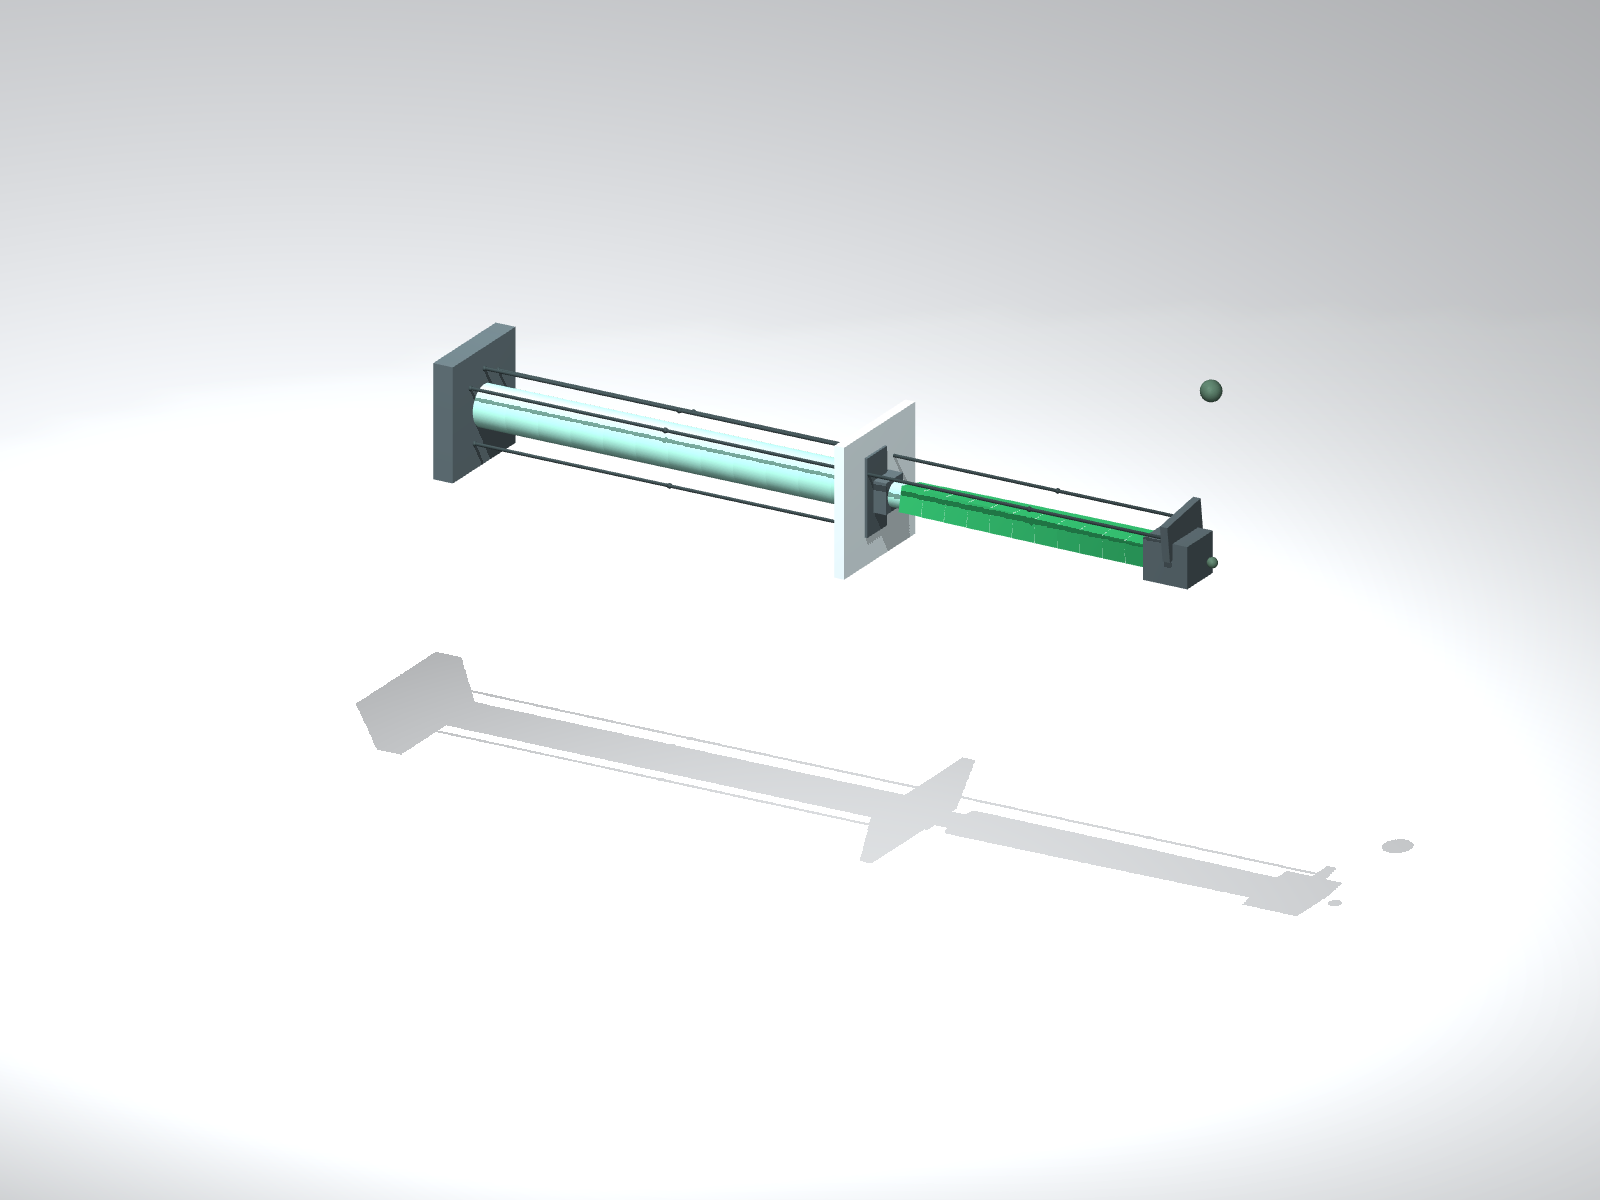
\includegraphics[width=\linewidth,height=0.60in,keepaspectratio]{figures/native/t07_round_root.png}\par
\scriptsize Refine the root and tendon route; re-optimize control.
&
\scriptsize One shared morphology satisfies four required conditions and 35 original hard constraints. The structural comparison is detailed in Fig.~\ref{fig:structure-evolution}.
\\
\midrule
\textbf{T10}
&
\centering
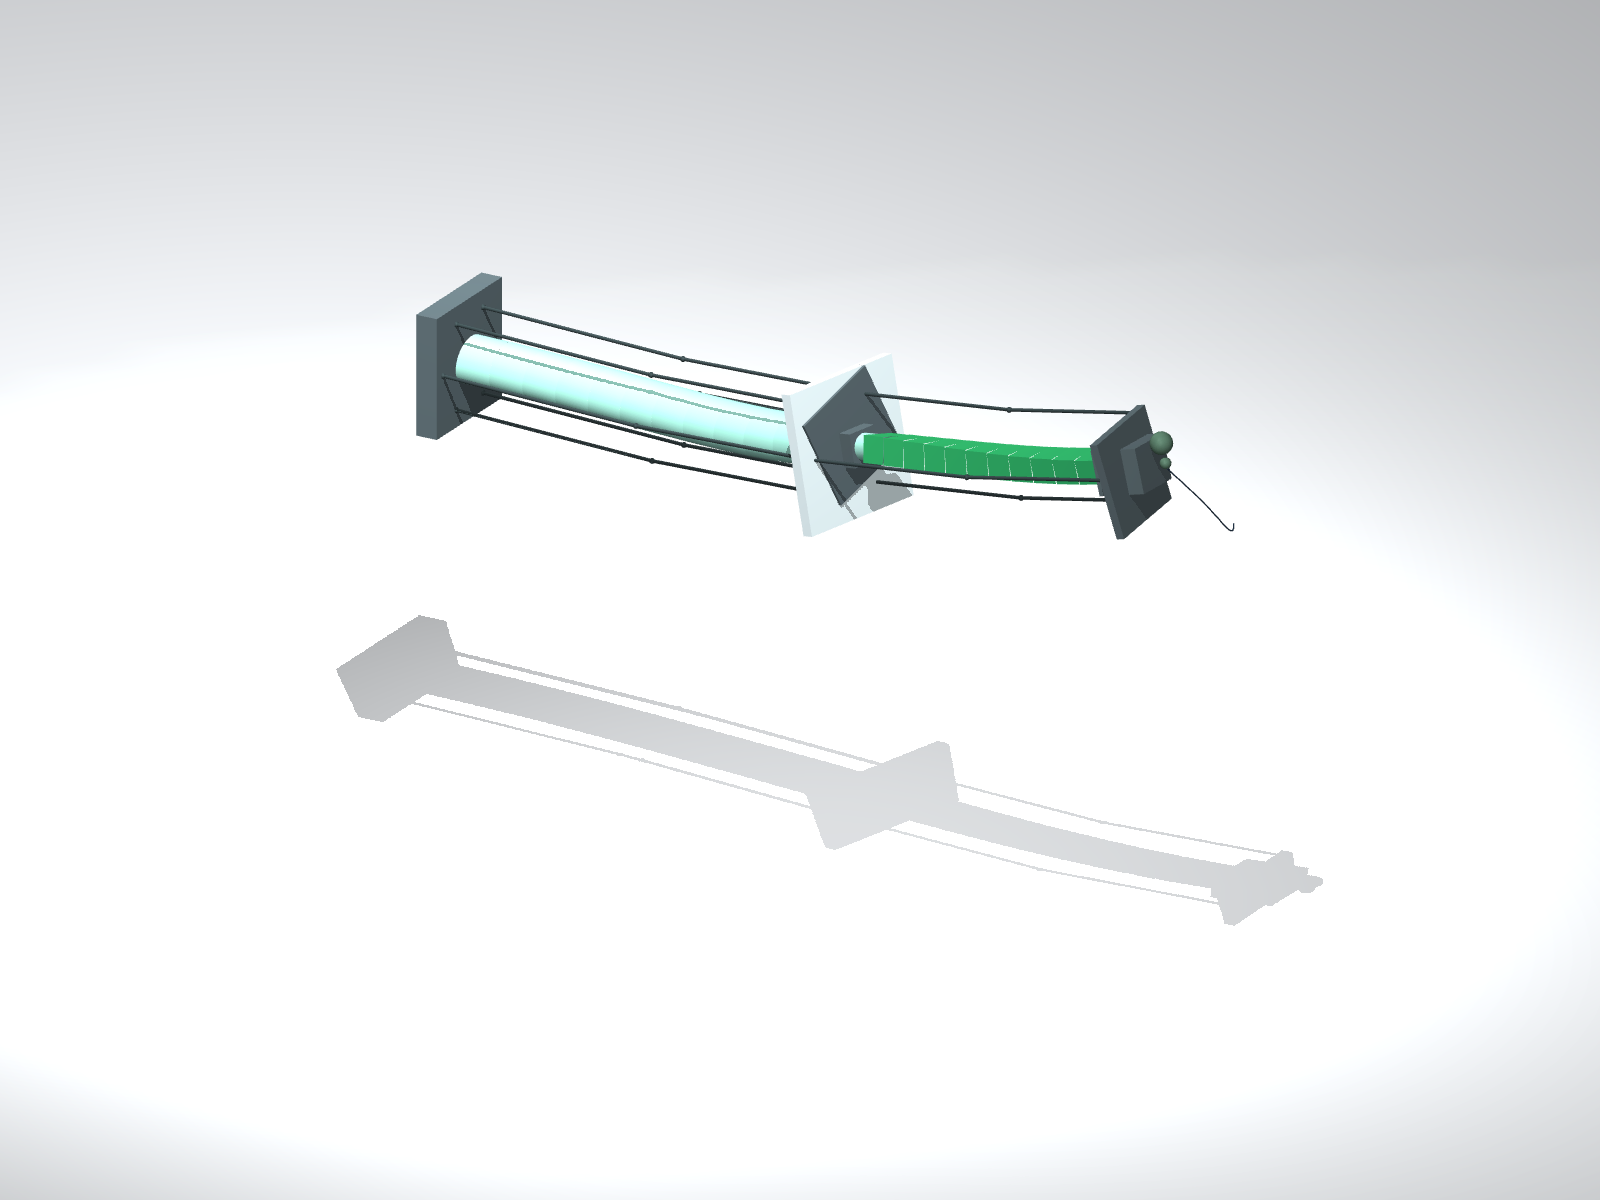
\includegraphics[width=\linewidth,height=0.60in,keepaspectratio]{figures/native/t10_preimpact.png}\par
\scriptsize GVS/NMPC trials retain recovery and tendon-limit conflicts.
&
\scriptsize The controller formulation is the bottleneck; the morphology can remain fixed.
&
\scriptsize Construct a native tangent model, discrete LQR, and bounded tension allocation.
&
\centering
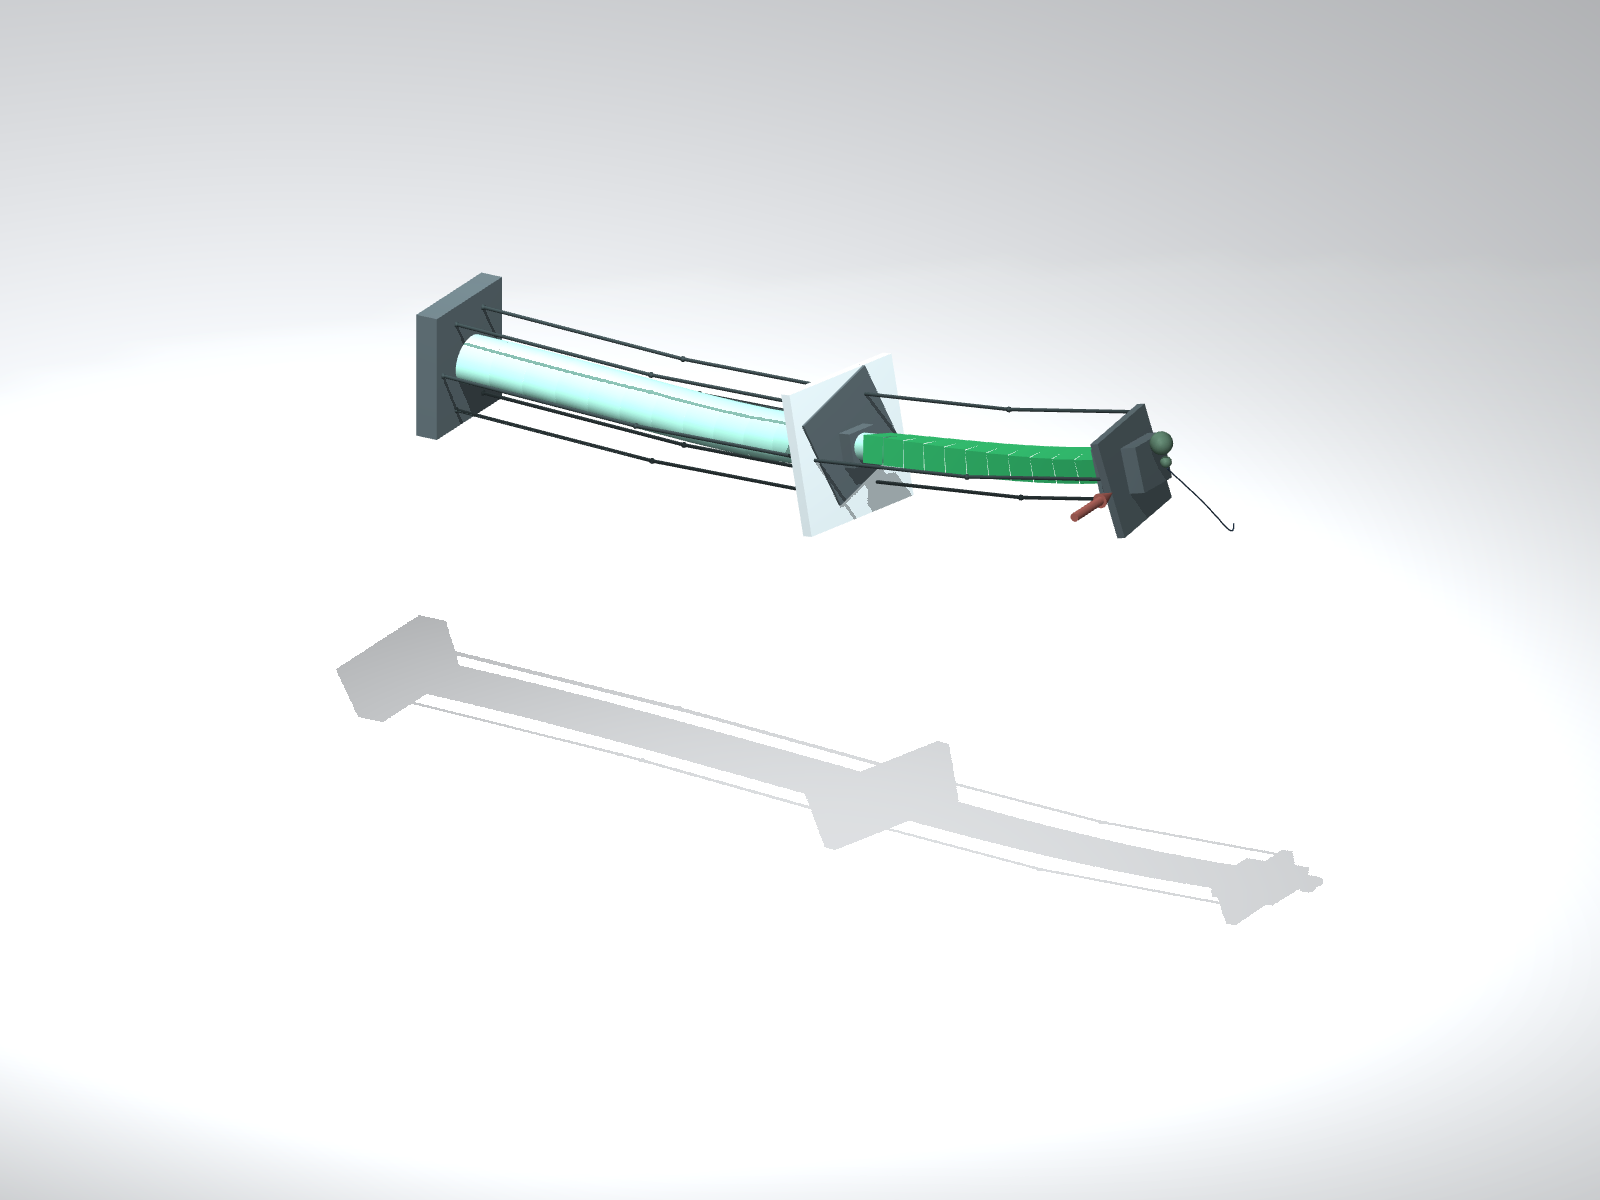
\includegraphics[width=.48\linewidth,height=0.60in,keepaspectratio]{figures/native/t10_impact.png}\hfill
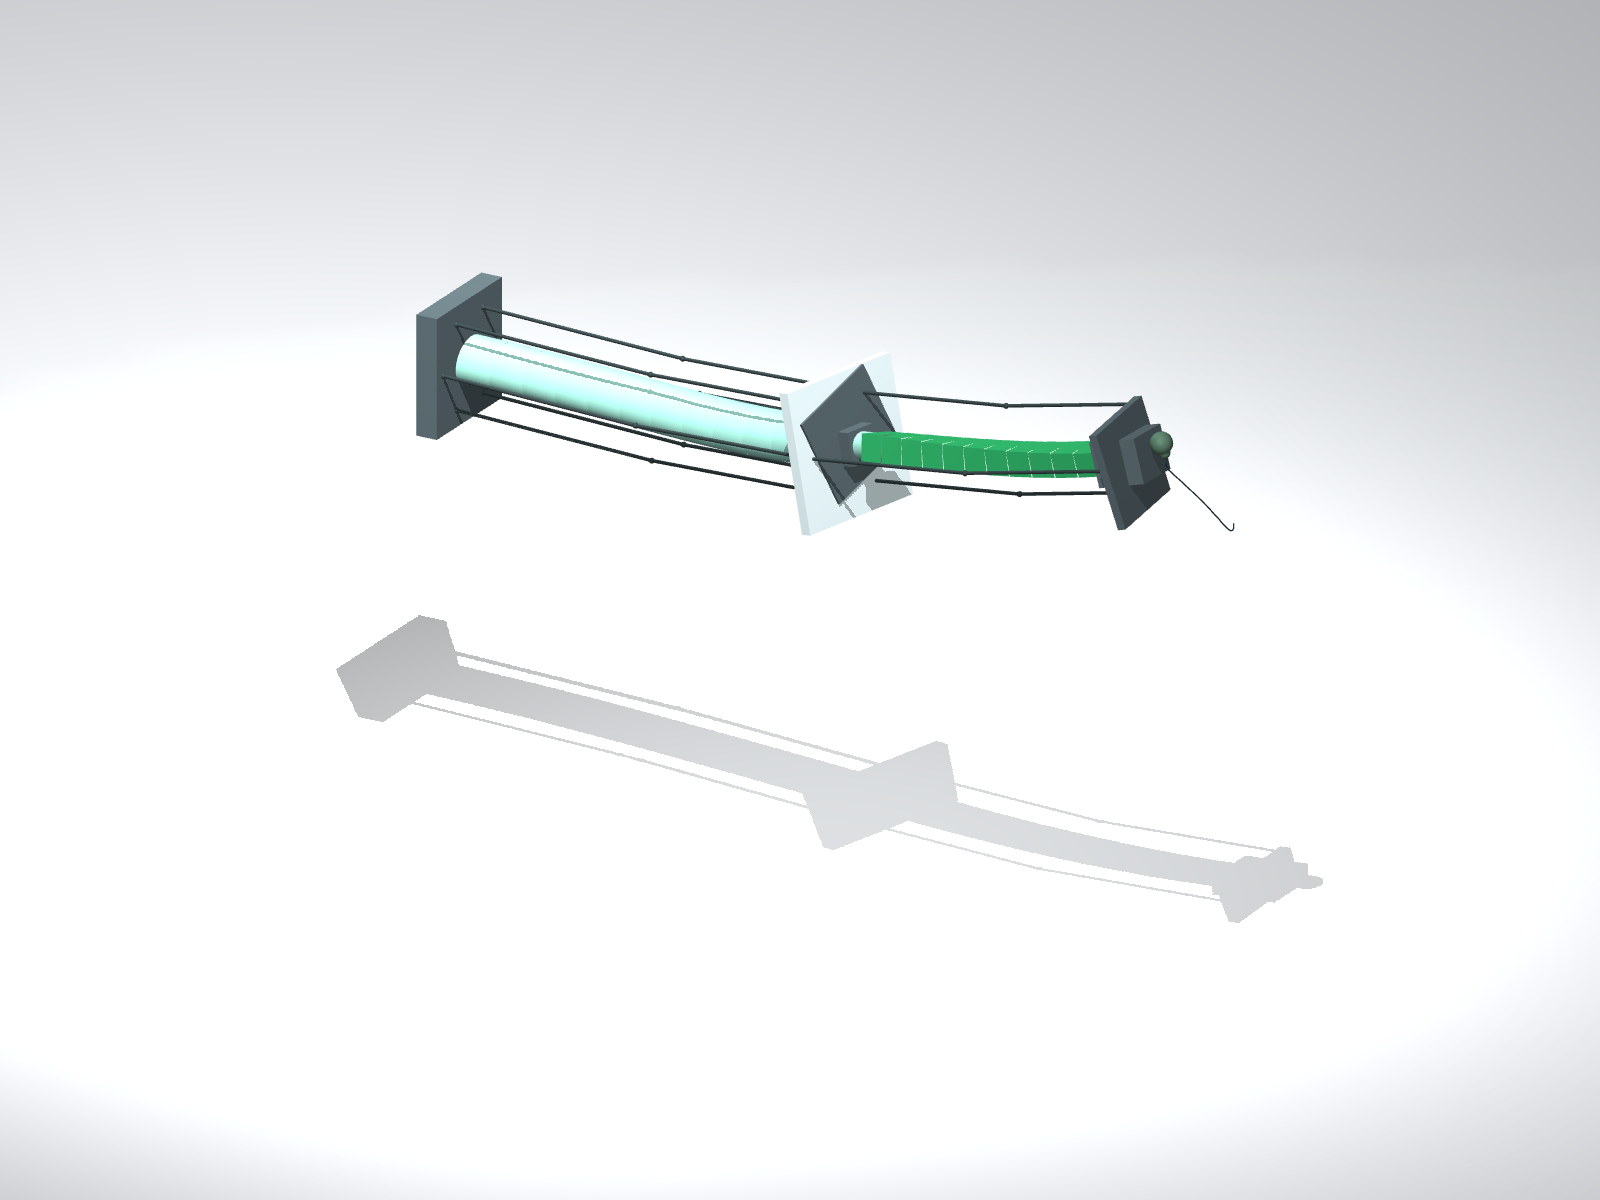
\includegraphics[width=.48\linewidth,height=0.60in,keepaspectratio]{figures/native/t10_final_hold.png}\par
\scriptsize Impact and recovered hold.
&
\centering
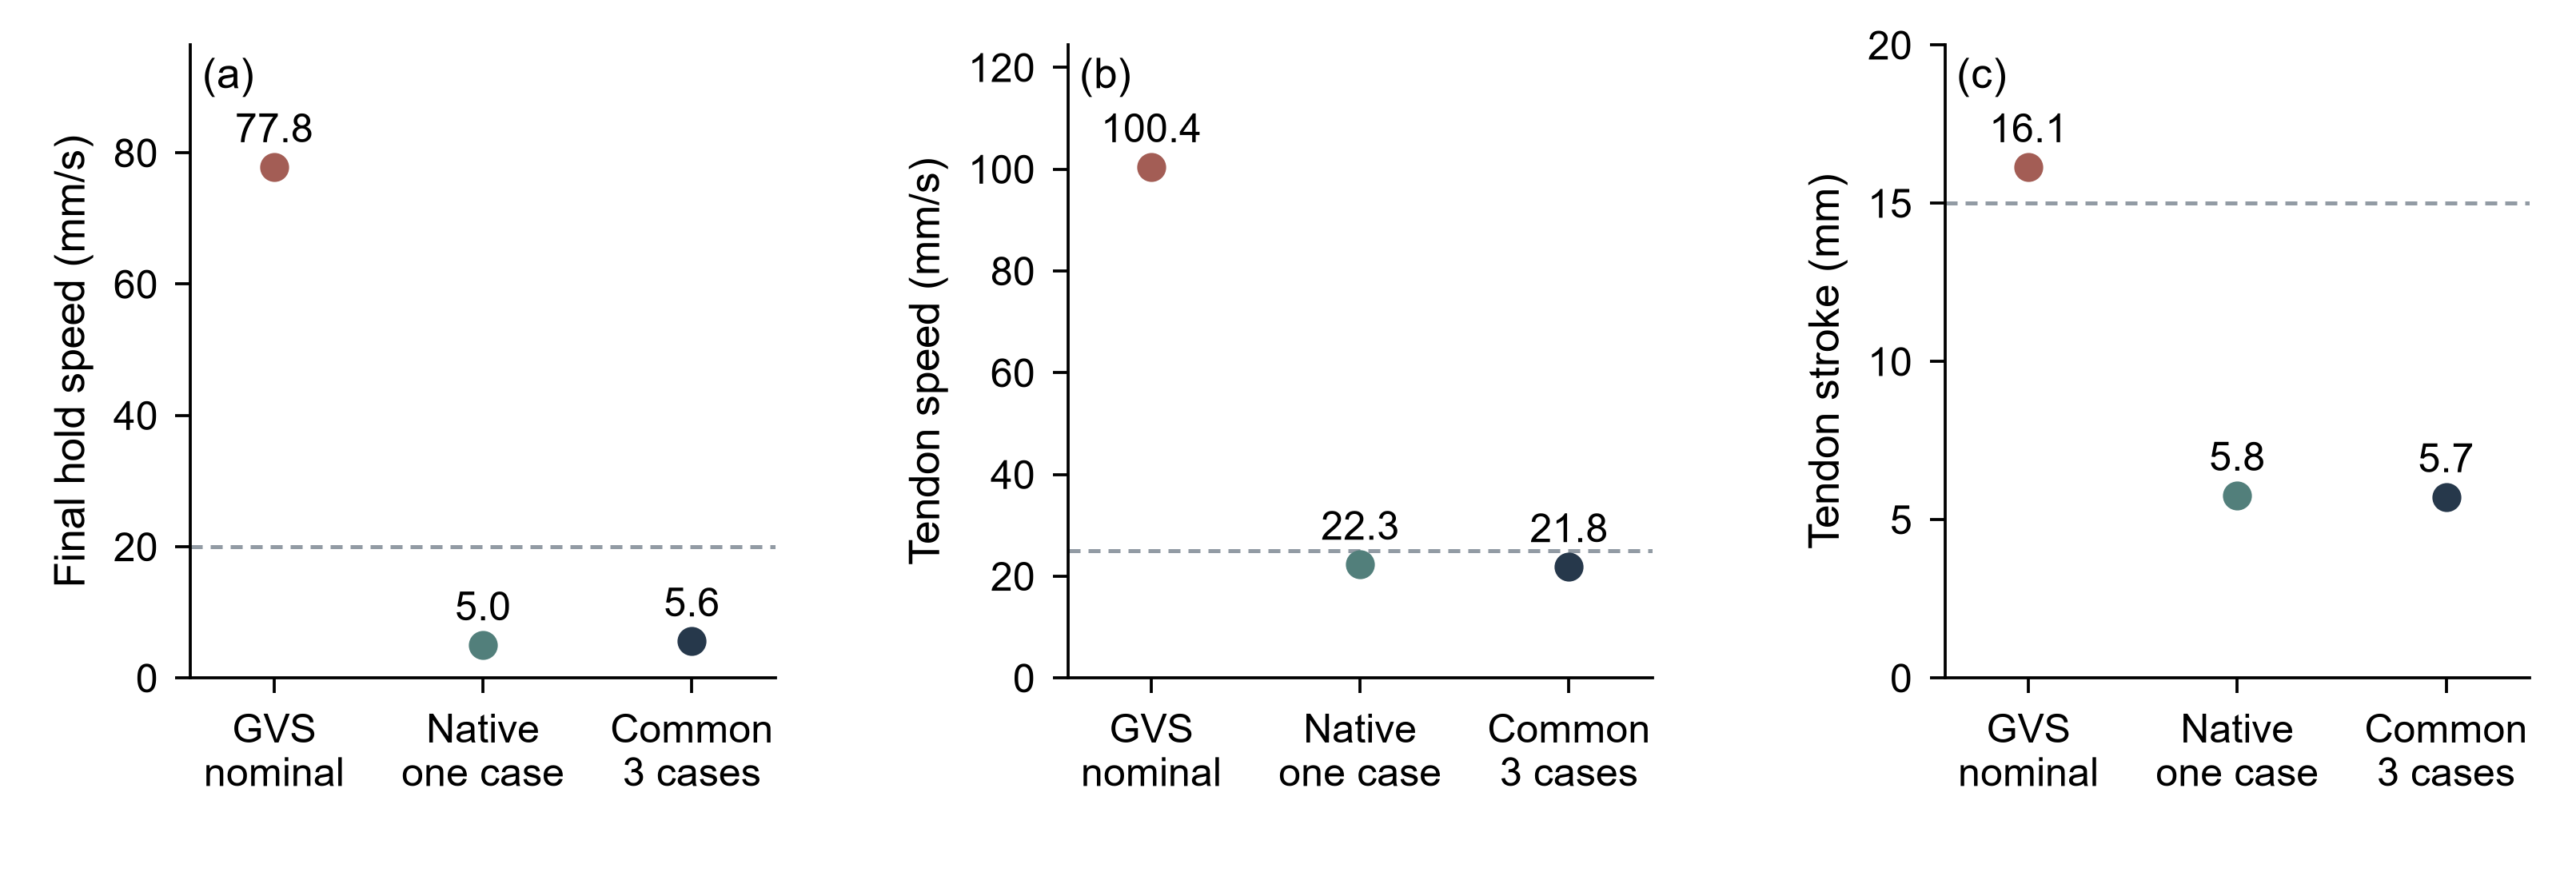
\includegraphics[width=\linewidth,height=0.60in,keepaspectratio]{figures/native/t10_control_comparison.png}\par
\scriptsize Common feedback: 3/3 required; frozen controls: 0/2.
\\
\bottomrule
\end{tabularx}
\par\vspace{4pt}
\noindent\textbf{Archive-level evidence-to-action trace}\par\vspace{2pt}
\begin{tikzpicture}[x=1cm,y=1cm]
\node[align=center] at (1.2,0.55) {\textbf{\large 220}\\[-1pt]\scriptsize Evidence-linked};
\draw[-{Stealth[length=2mm]},TraceSlate,line width=.8pt] (2.05,0.55)--(2.65,0.55);
\node[align=center] at (3.45,0.55) {\textbf{\large 205}\\[-1pt]\scriptsize Dispatched};
\draw[-{Stealth[length=2mm]},TraceSlate,line width=.8pt] (4.25,0.55)--(4.85,0.55);
\node[align=center] at (5.65,0.55) {\textbf{\large 160}\\[-1pt]\scriptsize Executed};
\draw[-{Stealth[length=2mm]},TraceSlate,line width=.8pt] (6.45,0.55)--(7.05,0.55);
\node[align=center] at (7.9,0.55) {\textbf{\large 10}\\[-1pt]\scriptsize Later independently\\[-2pt]\scriptsize PASS-linked};
\node[anchor=west,font=\scriptsize,text=TraceSlate] at (9.0,0.55) {72.73\% proposal-to-execution};
\end{tikzpicture}
\caption{Process-level dissection of adaptive research. The upper panel links recorded observations to physical hypotheses, investigations, research actions, and task outcomes; the lower strip summarizes the aggregate evidence-to-action trace. The counts are archive-level records under strict evidence/action/receipt linkage, and later independent validation is not interpreted as a causal effect or a general task success rate. Text is an editorial reconstruction of archived research decisions rather than a verbatim internal reasoning trace.}
\label{fig:process-dissection}
\end{figure*}
